   
        
        \begin{ledgroupsized}[r]{120mm}
        \footnotesize 
        \pstart        
        \noindent\textbf{\"{U}berlieferung:}  
        \pend
        \end{ledgroupsized}
      
       
              \begin{ledgroupsized}[r]{114mm}
              \footnotesize 
              \pstart \parindent -6mm
              \makebox[6mm][l]{\textit{L}}Konzept: LH XXXVIII Bl. 202. 2/3 Bog. 2\textsuperscript{o}, oben und unten beschnitten. 3~S., zweispaltig. Bl. 202r\textsuperscript{o} und 202~v\textsuperscript{o} umfassen jeweils vier Spalten. Textfolge: Spalte 1\textendash 4 von Bl. 202 r\textsuperscript{o}, Spalte 1\textendash 2 von Bl. 202 v\textsuperscript{o}. Spalte 3\textendash 4 von Bl. 202 v\textsuperscript{o} leer. Die Zeichnung \textit{[Fig. 1]} befindet sich im oberen Teil der Spalte 1 von Bl. 202 r\textsuperscript{o}. Darunter eine Erkl\"{a}rung von Johann Daniel Crafft. Die in Spalte 2 von Bl. 202 v\textsuperscript{o} befindliche Zeichnung \textit{[Fig. 2]} wurde durch sp\"{a}tere Erg\"{a}nzungen z.~T. \"{u}berschrieben.\\KK 1, Nr. 725\textsuperscript{a}, 725\textsuperscript{b} \pend
              \end{ledgroupsized}
        %\normalsize
        \vspace*{5mm}
        \begin{ledgroup}
        \footnotesize 
        \pstart
      \noindent\footnotesize{\textbf{Datierungsgr\"{u}nde}: Die Datierung ergibt sich aus der Erkl\"{a}rung von Johann Daniel Crafft auf Bl. 202 r\textsuperscript{o}, die als Datum der Unterzeichnung den 14. Juni 1671 ausweist.}
        \pend
        \end{ledgroup}
      
        \vspace*{8mm}
        \pstart 
        \normalsize
      [202 r\textsuperscript{o}] \selectlanguage{ngerman}Ich nachssbenanter bekenne dass mir heut dato H. Dr. Leibnitz\protect\index{Namensregister}{\textso{Leibniz} (Leibnitz), Gottfried Wilhelm (1646\textendash 1716)} gegenwertiges Vorhaben des Motus perpetui\protect\index{Sachverzeichnis}{motus!perpetuus} gezeiget. Verspreche hergegen, dafern etwas daran ist, ihme auch meine inuenta et experimenta bona fide zue communiciren. Vnd solle keiner von bejiden etwass demen andern zue schaden, sondern alles communicato consilio thun. Maÿntz den 14ten Junij 1671.\selectlanguage{latin}
      \pend
      \pstart Joh. Daniel Crafft manu propria\protect\index{Namensregister}{\textso{Crafft,} Johann Daniel 1624\textendash 1697} 
      \pend \vspace{1.0ex} 
      \pstart Esto vas aqua plenum \textit{abcd} \edtext{quantumcunque}{\lemma{}\Afootnote{quantumcunque \textit{ erg.} \textit{ L}}} in quo follis \textit{efgh} cujus pars inferior \textit{he} ex materia aqua graviore, ut plumbo\protect\index{Sachverzeichnis}{plumbum}: Pars superior \textit{gf} ex leviore ut ligno. Ita ut plus gravitet plumbum\protect\index{Sachverzeichnis}{plumbum}, quam levitet lignum, ac proinde plumbum\protect\index{Sachverzeichnis}{plumbum} contineat sub aqua lignum. Ponamus lignum esse dimidio levius aqua, plumbum\protect\index{Sachverzeichnis}{plumbum} decuplo gravius. Efficiamus eam rationem esse ligni ad plumbum\protect\index{Sachverzeichnis}{plumbum}, ut si paulo plus ligni accederet, vinceret lignum, nunc vincatur. Sunto enim: plumbum\protect\index{Sachverzeichnis}{plumbum} librarum decem, erit aqua paris spatii, librae unius; lignum librarum octo, erit aqua paris spatii librarum 16. Erit ergo follis totum pondus 18 librarum, aquae paris spatii 17 librarum, follis igitur totus summersus \edlabel{manebitstart}\edtext{manebit}{{\xxref{manebitstart}{manebitend}}\lemma{manebit.}\Afootnote{ \textit{ (1) }\ Efficiamus nunc ut ascendat sponte sua \textit{ (2) }\ Efficiamus nunc, [...] ascendat. \textit{ L}}}.
      \pend \clearpage
        \begin{center}
        \begin{tabular}{crrrrc||c}
        Follis pl. & 10 & \Pfund & lign. 8 & \Pfund & f. 18 & cavitas explicati \\
        capit Aquae & 1 & \textemdash & 16 & \textemdash & f. 17 & 6 (2) + 23 (19)
        \end{tabular}
        {\vrule height 0mm depth 10mm width 0mm}
        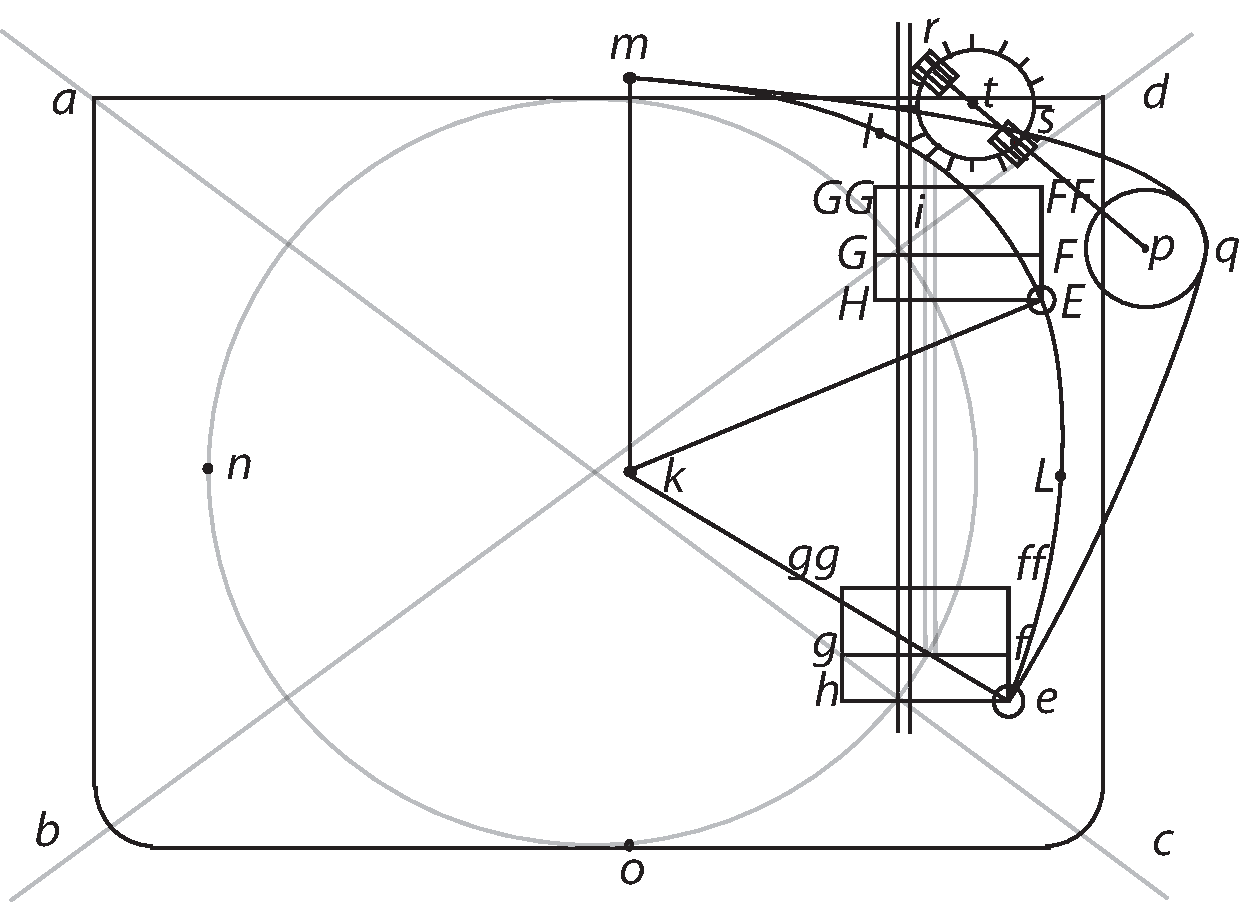
\includegraphics[width=1.0\textwidth]{images/38_202r}
        \\ \textit{[Fig. 1, tlw. Blindzeichnungen]}
        \end{center}
      \pstart Efficiamus nunc, ut 18 \Pfund\ follis, tantum occupent spatii, quantum 19 \Pfund\ et ultra, aquae, ac proinde follis in aqua ascendat\edlabel{manebitend}. Id fiet folle translato ex statu complicationis \textit{efgh} in statum explicationis \textit{effggh}. Explicabit autem ipse sese vi intrinseca\protect\index{Sachverzeichnis}{vis!intrinseca} hoc modo: Ponamus \textit{he} \edtext{plumbum\protect\index{Sachverzeichnis}{plumbum}}{\lemma{}\Afootnote{plumbum\protect\index{Sachverzeichnis}{plumbum} \textit{ erg.} \textit{ L}}} pessulo objecto ita esse firmatum, ut nec ascendere nec descendere possint in vase \textit{abcd}; contra, lignum \textit{fg} libere ascendere posse. Cumque sit 8 \Pfund, et proinde occupet spatium aquae 16 \Pfund\ 8 \Pfund\ aquae quibus ab ea superabitur conabuntur lignum elevare, seu levitatio ligni erit 8 \Pfund. Ascendendo explicabit follem eumque ponet in statu \textit{heffgg}. Sed quia explicando follem efficitur, ut tantum aquae loco cedere debeat, quantum est spatium a folle \edtext{explicato}{\lemma{}\Afootnote{explicato \textit{ erg.} \textit{ L}}} intus vacuo soloque aere, id est quantum ad nostram computationem nihilo, pleno, nunc occupatum, tantus erit renisus quantum cavitas explicati follis aquae caperet: Ponamus capere aquae libras 6 vel tantum 2 ut lubet satis magna enim hic latitudo eligendi permissa est. Ergo si ponis aquae libras 6. Renisus erit ut 6. \Pfund\ si libras 2 erit ut 2 \Pfund. Utervis superabitur a levitatione ligni, ut 8 \Pfund, ac proinde lignum poterit explicare follem \edtext{attracto aere per canalem non angustum ex folle sursum ultra summum aquae \textit{ad} in liberum aerem exeuntem.}{\lemma{}\Afootnote{attracto aere per canalem \textbar\ non angustum \textit{ erg.}\ \textbar\ ex folle [...] exeuntem. \textit{ erg.} \textit{ L}}} Follis explicatus si capit \edtext{cavitatem}{\lemma{}\Afootnote{cavitatem \textit{ erg.} \textit{ L}}} 6 \Pfund\ (2) pondere 18 \Pfund\ occupabit aquae 23 (19) \Pfund, ac proinde \edtext{totus, pessulo quod \textit{he} tenebat, ascendentis ligni potentia aperto, attolletur potentia 23 (19) \textendash\ 18 \Pfund\ hoc est potentia 5 (1) librarum (librae)}{\lemma{proinde}\Afootnote{ \textit{ (1) }\ potentia 23 (19) \textendash\ 18 \Pfund\ hoc est potentia 5 (1) librarum (librae) attolletur \textit{ (2) }\ totus, [...] (librae) \textit{ L}}} in lineis rectis \textit{eE}, \textit{hH}, \textit{ggGG}, \textit{hhHH} etc. ex loco \textit{heffgg} in locum\footnote{\textit{In H\"{o}he der folgenden Zeile in der ersten Spalte:} NB. Quod hic aqua, aliter aere fieri potest.} \textit{HEFFGG}. Possunt autem lineae \textit{eE} etc. esse quantaecunque, nam et vas \textit{abcd} est quantumcumque. Quam autem magnitudinem eligi satis sit, mox patebit. Cum igitur follis \edtext{explicatus}{\lemma{}\Afootnote{explicatus \textit{ erg.} \textit{ L}}} sit in loco superiore nunc quaerendum est quomodo complicatio ejus, ac descensus proinde rursus effici queat. Id ita fiet: \edtext{Plumbum\protect\index{Sachverzeichnis}{plumbum}}{\lemma{}\Afootnote{Plumbum\protect\index{Sachverzeichnis}{plumbum} \textit{ erg.} \textit{ L}}} \textit{HE} inciderit ascendendo in pessulum, ut nec sursum nec deorsum ire possit. Immineat pondus \textit{i} ligno \textit{GGFF} quod a pessulo quodam suo ascendentis ligni potentia liberatum circumacta ex qua pendet trochlea\protect\index{Sachverzeichnis}{trochlea} illabetur ligno \textit{GGFF} pondereque suo lignum ex loco explicationis \textit{GGFF}, deprimet in locum \edtext{complicationis}{\lemma{}\Afootnote{complicationis \textit{ erg.} \textit{ L}}} \textit{GF} aere per canalem eundem quo attractus est ex folle rursus expresso. Ad hoc praestandum, videamus quanta ei potentia opus sit. Ligni levitatio est 8 \Pfund\ per priora. Ea obtundetur a renisu aquae aerem expellere, seque in ejus locum reponere conantis ut 6 (2) \Pfund. Erit ergo ligni levitatio ut 2 (6) \Pfund. Poterit ergo pondus \textit{i} paulo amplius quam 2 (6) \Pfund\ esse, jamque sufficiet ad follem recomplicandum. Sed ne arctemus nos, et ut appareat libertas tanto major, esto pondus \textit{i} \Pfund\textsuperscript{ras} 9 recomplicabit sine controversia follem. Follis recomplicatus \edtext{rursus capiet}{\lemma{recomplicatus}\Afootnote{ \textit{ (1) }\ fiet \textit{ (2) }\ rursus capiet \textit{ L}}} tantum 17 \Pfund\ aquae, cum ipse ponderet 18, ac proinde aqua paris spatii gravior redescendet in locum priorem inferiorem. \pend \pstart Efficiendum autem ut redescensu suo, vel postea reascensu vel utroque simul, recollocet pondus \textit{i} in locum priorem. Etsi enim potentia follis non sit nisi 1 \Pfund\ in descendendo, 5 (1) \Pfund\ in ascendendo: Pondus autem \textit{i} sit 9 \Pfund\ ad summum \edtext{[quanquam sufficeret esse 3 (7) sed sinamus 9]}{\lemma{[...]}\Afootnote{\textit{Klammern von Leibniz}}} facile tamen ex communis mechanicae principiis follis attollet pondus \textit{i} quia magnitudo vasis \textit{abcd} potest esse quantacunque, ac proinde descensus ascensusque follis seu lineae \textit{eE}, \textit{hH} etc. quantaecunque. \edtext{Ascensus}{\lemma{quantaecunque.}\Afootnote{ \textit{ (1) }\ Jam \textit{ (2) }\ Ascensus \textit{ L}}} autem vel descensus ponderis \textit{i} non major quam quanta est altitudo cavitatis follis explicati, seu quanta est \textit{G,GG} quam possumus facere quantulam volumus. Quanto enim latior longiorque est follis, seu quanto major est recta \textit{HE}, tanto minorem necesse est esse altitudinem seu rectam \textit{G,GG} manente eadem capacitate. Constat autem ex communis mechanicae principiis, Machinarum debita applicatione effici posse, ut pondus minus vincat majus modo inter movendum tanto magis sit descensurum minus, quam ascensurum majus; quanto eo minus est: compensata per velocitatem parvitate. Id ergo in casu proposito sic fiet. 
      \pend 
      \pstart Descendat follis non in recta \textit{Ee}, sed in arcu \textit{LE} radio \textit{kL} vel \textit{kE} centro \textit{k}. Portionem trochleae\protect\index{Sachverzeichnis}{trochlea} (\edtext{\textit{ELmno}}{\lemma{trochleae}\Afootnote{ \textit{ (1) }\ \textit{elEmno} \textit{ (2) }\ (\textit{ELmno}) \textit{ L}}}) aequalem arcui \textit{elE} nempe \textit{Em} deferens secum in locum arcus \textit{elE}. Sit arcus \textit{Em} dentatus, circumagatque rotam \protect\index{Sachverzeichnis}{rota!dentata} \textit{pq} dentatam et ipsam, nisi malimus facilioris motus causa connectere filo \textit{mqe}, quo casu licebit dentibus carere ex \textit{p} in transversum exeat cylinder \textit{pr} duobus tympanis\protect\index{Sachverzeichnis}{tympanum} \edtext{dentatis}{\lemma{tympanis}\Afootnote{ \textit{ (1) }\ rotatis \textit{ (2) }\ dentatis \textit{ L}}} \textit{r} et \textit{s} incumbens rotae \textit{tr} in extremo utroque diametri \textit{r} et \textit{s}. Rota \protect\index{Sachverzeichnis}{rota!dentata} \textit{tr} sit dentata, sed interrupte, ita cum \edtext{tantum dentatum sit quantum tympanum incumbit, tantundem uno ascensu vel descensu morsurum est,}{\lemma{cum}\Afootnote{ \textit{ (1) }\ tantundem dentatum sit quantum tympanum\protect\index{Sachverzeichnis}{tympanum|textit} incumbit, tantum ex adverso sit interruptum \textit{ (2) }\ tantum [...] est, \textit{ L}}} sit vacuum. Ita fiet ut dum tympanum \protect\index{Sachverzeichnis}{tympanum} \textit{r} \edtext{imminet vacui parti, quam nec tangit}{\lemma{\textit{r}}\Afootnote{ \textit{ (1) }\ incumbit vacuo \textit{ (2) }\ imminet [...] tangit \textit{ L}}} nec quicquam rotatione cylindri \textit{rs} per rotationem rotae \textit{pq} ab arcu \textit{Em} procurata agit, tympanum \protect\index{Sachverzeichnis}{tympanum} \textit{s} incumbat dentatae, et agat suum. Arcusque \textit{Em} descendens agat tympano\protect\index{Sachverzeichnis}{tympanum} uno, ascendens opposito, atque ita utroque in eandem plagam\edtext{, quia}{\lemma{plagam}\Afootnote{ \textit{ (1) }\ . Idem sine interruptione certiore, puto, artificio fiet, si tympana\protect\index{Sachverzeichnis}{tympanum|textit} sint in baculo seu cylindro \textit{rs} mobilia \textit{(a)}\ ascendendoque intra limites praescriptos, \textit{(b)}\ ascendendoque unum, descendendo oppositum rotis incumbere efficiamus. Unum non totum exeat, \textit{(aa)}\ nisi initium jam \textit{(bb)}\ ante alterius ingressum, vel etiam, ut facilius tympana dentibus reinserantur efficiamus potius, ut modo hoc modo illud elevatum sit, ne dentes tangat. Optimus denique modus sine omni mutatione et perturbatione sui est. Sint tympana\protect\index{Sachverzeichnis}{tympanum|textit} tam grandia, ut toto descensu, vel toto ascensu non nisi semicircumferentia eorum circumeat. \textit{(aaa)}\ Semicircumferentia \textit{(bbb)}\ Pars magna circumagi debet cujusque sit una nuda altera dentibus armata; ita ut cum unius armata inferior est dentesque tangit alterius nuda inferior sit, ac proinde non tangat unoque, proinde descensu \textit{(aaaa)}\ rotationem \textit{(bbbb)}\ semirotationem unam absolvente, alterum ascensu alteram \textit{ (2) }\ , quia \textit{ L}}} opposito simul et loco et motu in eandem plagam \edtext{agat}{\lemma{plagam}\Afootnote{ \textit{ (1) }\ continuet \textit{ (2) }\ agat \textit{ L}}}. Nam si solus motus vel solus situs mutetur, contrarium; si uterque, idem evenit. Rotata jam rota \textit{tr} pondus sibi affixum \textit{i} reattollet. Quod ostendo. Ponamus trochleam\protect\index{Sachverzeichnis}{trochlea} \textit{pq} tantam esse, quanta est \textit{keE}, tympana\protect\index{Sachverzeichnis}{tympanum} \textit{r} et \textit{s} tam parva quam lubet, nihilominus quia trochleae\protect\index{Sachverzeichnis}{trochlea} \textit{pq} concentrica eodem tempore absolvent gyrum suum exiguum, quo trochlea\protect\index{Sachverzeichnis}{trochlea} \textit{ke} vel \textit{pq} magnum. Porro quo tempore tympanum\protect\index{Sachverzeichnis}{tympanum} absolvit \edtext{arcum}{\lemma{absolvit}\Afootnote{ \textit{ (1) }\ tantum sui \textit{ (2) }\ arcum \textit{ L}}} tot graduum, quot est arcus \textit{em}, id est postquam ascensus vel descensus absolutus est, toties mordeat rotam, \textit{tr} quantum necesse est ad pondus \textit{i} in locum priorem elevandum. Ita fiet ut \edtext{eodem aut rectius paulo minore tempore recollocetur in suum locum pondus}{\lemma{eodem}\Afootnote{ \textit{ (1) }\ tempore pondus \textit{ (2) }\ aut [...] pondus \textit{ L}}} \textit{i} et absolvat spatium parvum \textit{G,GG}, quo follis ascendit et ascendit, absolvitque spatium si volumus decuplo majus (nam in potestate est) \textit{eE} duplicatum.
      [202~v\textsuperscript{o}] Ergo \edtext{etsi follis gravitas in descensu, levitas in ascensu}{\lemma{etsi}\Afootnote{ \textit{ (1) }\ potentia follis \textit{ (2) }\ follis [...] ascensu \textit{ L}}} esset 1 \Pfund\ ponderis \textit{i} vero gravitas \edtext{9 \Pfund. Si}{\lemma{9 \Pfund.}\Afootnote{ \textit{ (1) }\ Cum \textit{ (2) }\ Si \textit{ L}}} tamen motus follis sit noncuplo celerior, aequiponderabunt, si decuplo, ut hic praeponderabit follis, attolletque pondus, quod erat faciendum. Nihil ergo video, quod ad machinae perfectionem desiderari possit. \edtext{Restituet enim motus}{\lemma{possit.}\Afootnote{ \textit{ (1) }\ Restituuntur enim omnia \textit{ (2) }\ Restituet enim motus \textit{ L}}} sibi situm priorem. Ergo causam suam. Effectus autem sibi restituens causam suam est perennis. Erit ergo motus machinae perennis\protect\index{Sachverzeichnis}{motus!perennis}. 
\pend 